\documentclass[12pt,a4paper,oneside]{report}
\usepackage{graphicx}
\usepackage{german,a4}
\usepackage{lmodern}
\usepackage{fancyhdr}
\usepackage[utf8]{inputenc}
%\usepackage{setspace}
\usepackage[T1]{fontenc}
\usepackage{hyperref}
\usepackage[sf]{titlesec}
\usepackage{textcomp}
\usepackage{makeidx}
\usepackage{amsmath}
%\usepackage[ngerman]{babel}
\usepackage{listings}
\usepackage{color}
\usepackage{colortbl}
\definecolor{lightgray}{rgb}{0.8,0.8,0.8}
\definecolor{darkgreen}{rgb}{0,0.6,0}
\usepackage{pdfpages}
\usepackage{graphicx}
\usepackage{cite}
\usepackage{listings}
\usepackage{array}
\usepackage{caption}
\usepackage{subcaption}
\usepackage[font=small,labelfont=bf]{caption}
\usepackage[utf8]{inputenc}
\usepackage[compat=1.0.0]{tikz-feynman}
\usepackage{mathtools}
% =====================================================
% Seite einrichten
% =====================================================
\setlength{\textwidth}{160mm} \setlength{\textheight}{235mm}
\setlength{\evensidemargin}{5mm} \setlength{\oddsidemargin}{5mm}
\setlength{\topmargin}{0mm} \setlength{\voffset}{-15mm}
\setlength{\headsep}{12mm} \setlength{\footskip}{15mm}
\setlength{\headheight}{15.1pt}

% =====================================================
% sonstige Einstellungen
% =====================================================
%\flushbottom % Textfluss schoen unten ausrichten
\footnotesep12pt % Abstand Text / Fussnote
%\setlength{\parindent}{0pt} \setlength{\abovecaptionskip}{-6pt}
%\setlength{\belowcaptionskip}{0pt} \setlength{\intextsep}{18pt}
%\renewcommand{\baselinestretch}{1.2} % Zeilenabstand
\setcounter{secnumdepth}{4}
\newcommand{\p}[1]{\texttt{#1}}
\nonfrenchspacing

% =====================================================
% Kopf- und Fusszeile formatieren
% =====================================================
\pagestyle{fancy}
\lhead[LE,RO]{\sf{\leftmark}}
\rhead[RE,LO]{\sf{\thepage}}
\lfoot{\setlength{\unitlength}{1mm}
\begin{picture}(0,0)
\put(0,-2){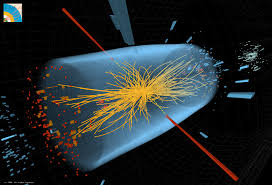
\includegraphics[height=0.6cm,width=0.8cm]{images/ppp.jpg}}
\end{picture}\put(10,2){\scriptsize\sf{Institut for theoretical physics}}\put(10,-2){\scriptsize\sf{Karlsruher institut for Technology (KIT)}}}
\cfoot{}
\rfoot{\footnotesize\sf{Thesis by Tigran Saidnia}}
\renewcommand{\headrulewidth}{0.4pt}
\renewcommand{\footrulewidth}{1.0pt}
\newcommand{\offline}{$ \overline{\textrm{\textbf{Off}}}\underline{\textrm{\textbf{line}}}\ $}


% ====================================================
% Kopf- und Fusszeile fuer "plain"-Format ueberschreiben
% ====================================================
\fancypagestyle{plain}{%
\fancyhf{}
\fancyfoot[L,C,R]{\setlength{\unitlength}{1mm}
\begin{picture}(0,0)
\put(0,-2){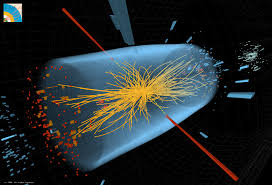
\includegraphics[height=0.6cm,width=0.8cm]{images/ppp.jpg}}
\end{picture}\put(10,2){\scriptsize\sf{Institut for theoretical physics}}\put(10,-2){\scriptsize\sf{Karlsruhe Institut of Technology (KIT)}}}
\cfoot{}
\rfoot{\footnotesize\sf{Thesis by Tigran Saidnia}}
\renewcommand{\headrulewidth}{0pt}
\renewcommand{\footrulewidth}{1.0pt}}

\begin{document}

%\doublespacing
    \parindent=0pt
    %\sloppypar
    \linespread{1.2}
    \thispagestyle{plain}
    %\frontmatter
    %\maketitle

\begin{titlepage}

\begin{center}


% Oberer Teil der Titelseite:

\includegraphics[width=0.3\textwidth]{images/Intro/kitlogo_de_rgb}\\[1cm]    

\textsc{\LARGE Master Thesis}\\[0.5cm]
\textsc{\Large by}\\[0.5cm]
\textsc{\Large Tigran Saidnia}\\[1.0cm]


% Title
\newcommand{\HRule}{\rule{\linewidth}{0.5mm}}
\HRule \\[0.8mm]
{\textbf{\Large \bfseries Emission kernels of parton showers in LO}}\\[0.8mm]

%\HRule \\[0.001mm]
%\newcommand{\HRule}{\rule{\linewidth}{0.5mm}}
%\HRule \\[0.8mm]
%{\textbf{\bfseries Emission kernels of parton showers in LO}}\\[0.8mm]

\HRule \\[1cm]
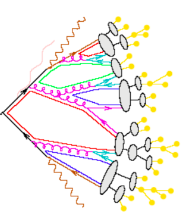
\includegraphics[scale=0.7]{images/Intro/footPicture.PNG}\\[0.8cm]   

\Large Karlsruhe institute of Technology (KIT)\\[1.5mm]
\Large Institute for theoretical physics\\[1.0cm]

{\Large Reviewer: PD Dr. Stefan Gieseke \\
\Large Second reviewer: Prof. Dr. Dieter Zeppenfeld\\
\Large External advisor: Dr. Simon Plätzer\\
\Large Advisor: Emma Simpson Dore}\\[0.8cm]   

Duration: July 1, 2018  –  July 1, 2019

\vfill

% Unterer Teil der Seite
 %\today

\end{center}

\end{titlepage}
\chapter*{}
\begin{flushleft}
\vspace{11cm}
\textbf{Statement of Originality}\\[1cm]
I hereby confirm that I have written the accompanying thesis by myself, without contributions from any sources other than those cited in the text and acknowledgements. This applies also to all graphics, drawings, maps and images included in the thesis.\\[1cm]

Karlsruhe, \today \\[1cm]
\end{flushleft}

\begin{center}
---------------------------------\\
Tigran Saidnia
\end{center}

\pagebreak

\tableofcontents
\thispagestyle{empty}
\addcontentsline{toc}{chapter}{Literaturverzeichnis}
\thispagestyle{empty}
\quad
\newpage
\pagenumbering{arabic} 




\input{abstract/abtract.tex}
\newpage
\section{Old parametrisation}

	
\begin{equation}
	\left.\begin{aligned}
	&{q_i}^{\mu} = z{p_i}^{\mu} + y(1-z){p_j}^{\mu} + \sqrt{zy(1-z)}{m}_{\bot} \\
	&{q}^{\mu}   = (1-z){p_i}^{\mu} + yz {p_j}^{\mu} - \sqrt{zy(1-z)}{m}_{\bot} \\
	&{q_j}^{\mu} = (1-y) {p_j}^{\mu} \\
		&y       = \frac{q_i q}{p_i p_j} \\
&q_i +q      = p_i + yp_j \\
&q_j +q      = (1-z){p_i}^{\mu} + (1+yz-y) {p_j}^{\mu} - \sqrt{zy(1-z)}{m}_{\bot}\\
&q_i \cdot q = y(1-2z+2z^2)(p_i \cdot p_j)\\
&q_i \cdot q_j = z(1-y) (p_i \cdot p_j)\\
&q_j \cdot q = (1-z)(1-y) (p_i \cdot p_j)
		\end{aligned}
	\right\}
	\quad \text{parametrisation}
\end{equation}


\section{new kinematic}
For the general m emission case it must be defined a new mapping. The parametrisation of the splitting momenta is formalized as:
\begin{equation}
	\begin{split}
	&{k_l}^{\mu} = \alpha_l \alpha {\Lambda^{\mu}}_{\nu}{p_i}^{\nu} + y\beta{n}^{\mu} + \sqrt{y\alpha_l\beta_l}{n^{\mu}}_{\bot,l} \:\:\:\:\:\:\:\:\:\:\:\:\:\:\:{l=1,...,m} \\
	&{q_i}^{\mu}   = (1-\displaystyle\sum\limits_{l=1}^m \alpha_l) \alpha {\Lambda^{\mu}}_{\nu}{p_i}^{\nu} + y(1-\displaystyle\sum\limits_{l=1}^m \beta_l){n}^{\mu} - \sqrt{y\alpha_l\beta_l}{n^{\mu}}_{\bot,l} \\
	&{q_k}^{\mu} = \alpha {\Lambda^{\mu}}_{\nu}{p_k}^{\nu} \:\:\:\:\:\:\:\:\:\:\:\:\: {k=1,...,n}\:\:\:\:\:\:\:\:\:\:k\neq i\\
    \end{split}
\end{equation}
$ k = 1,...,n $ labels the emission momenta and is taken to be massless $ {k_l}^2 = 0 $. Where the label $ l $ denotes the count of emissions. In this work we just want to considerate the one-emission kernels. The other important issue here is that all hard momenta are on-shell, $ {p_k}^2={q_k}^2=0 $.\\
to absorb the recoil we define $ n^{\mu} $ as:

\begin{equation}
\begin{split}
{n^{\mu}} &= Q^{\mu}-\frac{Q^2}{2p_i \cdot Q} {p_i}^{\mu}
\end{split}	
\end{equation}

Whereby Q is the total momentum with:

\begin{equation}
\begin{split}	
{Q}^{\mu} &= {q_i}^{\mu}+\displaystyle\sum\limits_{l=1}^m k_l^{\mu}+\displaystyle\sum\limits_{k=1}^m q_k^{\mu}={p_i}^{\mu}+\displaystyle\sum\limits_{k=1}^m p_k^{\mu}
\end{split}	
\end{equation}
To fulfil the condition that the emission momenta are massless, we need the following condition:

\begin{equation}
\begin{split}
	{n^{\mu}}_{\bot,l}{\Lambda^{\mu}}_{\nu}{p_i}^{\nu} &= {n_{\bot,l}} \cdot n = {n_{\bot,l}} \cdot Q =0\\
	{n^{\mu}}_{\bot,l}\cdot p_k &\neq0\\
\end{split}	
\end{equation}

$ {n}^2_{\bot,l} = -2\alpha{\Lambda^{\mu}}_{\nu}{p_i}^{\nu} n_{\mu} $ is not on-shell and in terms of single emission case we get $ {n}^2_{\bot,1} = -2p_i\cdot Q $.
The parameter y is related to the virtuality of the splitting parton:

\begin{equation}
\begin{split}
{q_i}^{\mu} +\displaystyle\sum\limits_{l=1}^m k_l^{\mu}   &= \alpha{\Lambda^{\mu}}_{\nu}{p_i}^{\nu} +y{n}^{\mu}\\
    \end{split}
\end{equation}
With $ \alpha = \sqrt{1-y} $.
\subsubsection*{Lorenz trafo}
In order to be able to work with the parametrisation, we have to do the Lorenz transformation of the Emitters, Spectator and total momentum first.

\begin{equation}
\begin{split}	
&\alpha{\Lambda^{\mu}}_{\nu} = {p_i}^{\mu} p_{i\nu} \frac{-y^2 Q^2}{4(p_i\cdot Q)^2(1+\sqrt{1-y}-\frac{y}{2})}
+{p_i}^{\mu} Q_{\nu} \frac{y(1+\sqrt{1-y})}{2(p_i\cdot Q)(1+\sqrt{1-y}-\frac{y}{2})}\\
&+{Q}^{\mu} p_{i\nu} \frac{(y^2 -y-y\sqrt{1-y})}{2(p_i\cdot Q)(1+\sqrt{1-y}-\frac{y}{2})}+\sqrt{1-y} {\eta^{\mu}}_{\nu}\\
\end{split}
\end{equation}

In the collinear limit of $ y \rightarrow 0, \alpha \rightarrow 1 $
this transformation reduces to trivial $ {\eta^{\mu}}_{\nu} $.


\begin{equation}
\begin{split}
&{\hat{{p_i}}}^{\mu}=\alpha{\Lambda^{\mu}}_{\nu} {p_i}^{\nu}= {p_i}^{\mu} p_{i\nu}{p_i}^{\nu} \frac{-y^2 Q^2}{4(p_i\cdot Q)^2(1+\sqrt{1-y}-\frac{y}{2})}
	+{p_i}^{\mu} Q_{\nu}{p_i}^{\nu} \frac{y(1+\sqrt{1-y})}{2(p_i\cdot Q)(1+\sqrt{1-y}-\frac{y}{2})}\\
&+{Q}^{\mu} p_{i\nu}{p_i}^{\nu} \frac{(y^2 -y-y\sqrt{1-y})}{2(p_i\cdot Q)(1+\sqrt{1-y}-\frac{y}{2})}+\sqrt{1-y} {\eta^{\mu}}_{\nu}{p_i}^{\nu}\\
\end{split}
\end{equation}

\begin{equation}
\begin{split}
&{\hat{{p_i}}}^{\mu}={p_i}^{\mu} (Q\cdot p_i) \frac{y(1+\sqrt{1-y})}{2(p_i\cdot Q)(1+\sqrt{1-y}-\frac{y}{2})}+\sqrt{1-y} {p_i}^{\mu}\\
&={p_i}^{\mu} [ \frac{y(1+\sqrt{1-y})}{(2+2\sqrt{1-y}-y)}+\sqrt{1-y}]={p_i}^{\mu}
    \end{split}
\end{equation}

\begin{equation}
	\begin{aligned}
		\fbox{$  {\hat{{p_i}}}^{\mu}=\alpha{\Lambda^{\mu}}_{\nu} {p_i}^{\nu}= {p_i}^{\mu}$}
    \end{aligned}
\end{equation}

\begin{equation}
	\begin{aligned}
	{\hat{{p_k}}}^{\mu}=\alpha{\Lambda^{\mu}}_{\nu} {p_k}^{\nu}= {p_i}^{\mu} p_{i\nu}{p_k}^{\nu} \frac{-y^2 Q^2}{4(p_i\cdot Q)^2(1+\sqrt{1-y}-\frac{y}{2})}
	+{p_i}^{\mu} Q_{\nu}{p_k}^{\nu} \frac{y(1+\sqrt{1-y})}{2(p_i\cdot Q)(1+\sqrt{1-y}-\frac{y}{2})}\\
	+{Q}^{\mu} p_{i\nu}{p_k}^{\nu} \frac{(y^2 -y-y\sqrt{1-y})}{2(p_i\cdot Q)(1+\sqrt{1-y}-\frac{y}{2})}+\sqrt{1-y} {\eta^{\mu}}_{\nu}{p_k}^{\nu}\\
    \end{aligned}
\end{equation}

\begin{equation}
	\begin{aligned}
	{\hat{{p_k}}}^{\mu}=\alpha{\Lambda^{\mu}}_{\nu} {p_k}^{\nu}= {p_i}^{\mu}[  \frac{-y^2 Q^2 (p_{i}\cdot {p_k})}{4(p_i\cdot Q)^2(1+\sqrt{1-y}-\frac{y}{2})}+ \frac{y(1+\sqrt{1-y})(Q \cdot {p_k})}{2(p_i\cdot Q)(1+\sqrt{1-y}-\frac{y}{2})}]\\
	+{Q}^{\mu} [ \frac{(y^2 -y-y\sqrt{1-y}) (p_{i}\cdot {p_k})}{2(p_i\cdot Q)(1+\sqrt{1-y}-\frac{y}{2})}]
	+\sqrt{1-y} {p_k}^{\mu}\\
    \end{aligned}
\end{equation}


\begin{equation}
	\begin{aligned}
	{\hat{{p_k}}}^{\mu}&=\alpha{\Lambda^{\mu}}_{\nu} {p_k}^{\nu}= {p_i}^{\mu}[  \frac{-y^2 Q^2 (p_{i}\cdot {p_k})}{4(p_i\cdot Q)^2(1+\sqrt{1-y}-\frac{y}{2})}+ \frac{y(1+\sqrt{1-y})(Q \cdot {p_k})}{2(p_i\cdot Q)(1+\sqrt{1-y}-\frac{y}{2})}]\\
	&+{Q}^{\mu} [ \frac{(y^2 -y-y\sqrt{1-y}) (p_{i}\cdot {p_k})}{2(p_i\cdot Q)(1+\sqrt{1-y}-\frac{y}{2})}]+\sqrt{1-y} {p_k}^{\mu}\\	
\text{with}\\
	A_1 &\equiv  \frac{-y^2 Q^2 (p_{i}\cdot {p_k})}{4(p_i\cdot Q)^2(1+\sqrt{1-y}-\frac{y}{2})}+ \frac{y(1+\sqrt{1-y})(Q \cdot {p_k})}{2(p_i\cdot Q)(1+\sqrt{1-y}-\frac{y}{2})}\\
		A_2 &\equiv   \frac{(y^2 -y-y\sqrt{1-y}) (p_{i}\cdot {p_k})}{2(p_i\cdot Q)(1+\sqrt{1-y}-\frac{y}{2})}\:\:\:\:\:\:\:\:\:\:\:\:\:\:\:\:\:\:\:\:\:\:\:\:\:\:\:\:\:\:\:\:\:\:\:\:\:\:\:\:\:\:\:\:\:\:\:\:\:\:\:\:\:\:\\\
    \end{aligned}    
\end{equation}
\begin{equation}
	\begin{aligned}
		\fbox{$  {\hat{{p_k}}}^{\mu}= A_1 \:{p_i}^{\mu}+A_2\:{Q}^{\mu}+\sqrt{1-y} {p_k}^{\mu} $}
    \end{aligned}
\end{equation}


\begin{equation}
	\begin{aligned}
	{\hat{{Q}}}^{\mu}&=\alpha{\Lambda^{\mu}}_{\nu} {Q}^{\nu}= {p_i}^{\mu}[  \frac{-y^2 Q^2 (p_{i}\cdot {Q})}{4(p_i\cdot Q)^2(1+\sqrt{1-y}-\frac{y}{2})}+ \frac{y(1+\sqrt{1-y})Q^2}{2(p_i\cdot Q)(1+\sqrt{1-y}-\frac{y}{2})}]\\
	&+{Q}^{\mu} [ \frac{(y^2 -y-y\sqrt{1-y}) (p_{i}\cdot {Q})}{2(p_i\cdot Q)(1+\sqrt{1-y}-\frac{y}{2})}]
	+\sqrt{1-y} {Q}^{\mu}\\
\text{with}\\
	S_1 &\equiv  \frac{Q^2}{2p_i \cdot Q}[\frac{-y^2}{2(1+\sqrt{1-y}-\frac{y}{2})}+ \frac{y(1+\sqrt{1-y})}{(1+\sqrt{1-y}-\frac{y}{2})}]=\frac{Q^2}{2p_i \cdot Q}y\\
		S_2 &\equiv   \frac{(y^2 -y-y\sqrt{1-y})}{2(1+\sqrt{1-y}-\frac{y}{2})}+\sqrt{1-y}=1-y\:\:\:\:\:\:\:\:\:\:\:\:\:\:\:\:\:\:\:\:\:\:\:\:\:\:\:\:\:\:\:\:\:\:\:\:\:\:\:\:\:\:\:\:\:\:\:\:\:\:\:\:\:\:\\\	
    \end{aligned}    
\end{equation}
\begin{equation}
	\begin{aligned}
		\fbox{$  {\hat{{Q}}}^{\mu}= \frac{Q^2}{2p_i \cdot Q}y \:{p_i}^{\mu}+(1-y)\:{Q}^{\mu} $}
    \end{aligned}
\end{equation}

\section{Single emission part}
\begin{equation}
	\begin{aligned}
	{k_1}^{\mu} &= (\alpha_1 -y\beta_1(\frac{Q^2}{2p_i \cdot Q})) {p_i}^{\mu} + y\beta_1{Q}^{\mu} + \sqrt{y\alpha_1\beta_1}{n^{\mu}}_{\bot,1}  \\
	{q_i}^{\mu}   &= (\beta_1 -\alpha_1 y(\frac{Q^2}{2p_i \cdot Q})){p_i}^{\mu} + y\alpha_1{Q}^{\mu} - \sqrt{y\alpha_1\beta_1}{n^{\mu}}_{\bot,l} \\
	{q_k}^{\mu} &= \alpha {\Lambda^{\mu}}_{\nu}{p_k}^{\nu} \:\:\:\:\:\:\:\:\:\:\:\:\: {k=1,...,n}\:\:\:\:\:\:\:\:\:\:k\neq i\\
	\\
	\\
		{k_1}^{\mu} &= \zeta_1 {p_i}^{\mu} + \lambda_1{Q}^{\mu} + \sqrt{y\alpha_1\beta_1}{n^{\mu}}_{\bot,1}  \\
	{q_i}^{\mu}   &= \zeta_q{p_i}^{\mu} + \lambda_q{Q}^{\mu} - \sqrt{y\alpha_1\beta_1}{n^{\mu}}_{\bot,l} \\
	{q_k}^{\mu} &= A_1{p_i}^{\mu} + A_2{Q}^{\mu} + \sqrt{1-y}{p_k^{\mu}}\\
    \end{aligned}
\end{equation}

\begin{equation}
	\begin{aligned}
	\zeta_1\zeta_1=({\alpha_1}^2 -2y\alpha_1 \beta_1(\frac{Q^2}{2p_i \cdot Q})+y^2{\beta_1}^2(\frac{Q^2}{2p_i \cdot Q})^2)\\
	\zeta_1\lambda_1=(y\alpha_1\beta_1 -{y^2\beta_1}^2(\frac{Q^2}{2p_i \cdot Q}))\\
	\zeta_1\zeta_q=(\alpha_1\beta_1-y({\alpha_1}^2+{\beta_1}^2) (\frac{Q^2}{2p_i \cdot Q})+y^2{\alpha_1}{\beta_1}(\frac{Q^2}{2p_i \cdot Q})^2)\\
	\zeta_1\lambda_q=(y{\alpha_1}^2 -y^2\beta_1\alpha_1(\frac{Q^2}{2p_i \cdot Q}))\\
	\zeta_q\zeta_q=	({\beta_1}^2 -2y\alpha_1\beta_1 (\frac{Q^2}{2p_i \cdot Q})+ y^2{\alpha_1}^2 (\frac{Q^2}{2p_i \cdot Q})^2) \\
	\zeta_q\lambda_1=(y{\beta_1}^2 -y^2\alpha_1 \beta_1(\frac{Q^2}{2p_i \cdot Q}))\\
	\zeta_q\zeta_1=(\beta_1\alpha_1-y({\beta_1}^2+{\alpha_1}^2)(\frac{Q^2}{2p_i \cdot Q})+y^2\alpha_1\beta_1 (\frac{Q^2}{2p_i \cdot Q})^2)\\
	\zeta_q\lambda_q=(y\beta_1\alpha_1 -y^2{\alpha_1}^2(\frac{Q^2}{2p_i \cdot Q}))\\
	\lambda_1\lambda_1=y^2{\beta_1}^2\\
	\lambda_1\zeta_q=(y{\beta_1}^2 -y^2\alpha_1 \beta_1(\frac{Q^2}{2p_i \cdot Q}))\\
	\lambda_1\lambda_q=y^2\beta_1\alpha_1\\
	\lambda_1\zeta_1=(y\beta_1\alpha_1 -y^2{\beta_1}^2(\frac{Q^2}{2p_i \cdot Q}))\\
	\lambda_q\lambda_q=y^2{\alpha_1}^2\\
	\lambda_q\lambda_1=y^2\alpha_1\beta_1\\
	\lambda_q\zeta_q=(y\alpha_1\beta_1 -y^2{\alpha_1}^2 (\frac{Q^2}{2p_i \cdot Q}))\\
	\lambda_q\zeta_1=(y{\alpha_1}^2 -y^2\alpha_1\beta_1(\frac{Q^2}{2p_i \cdot Q}))
    \end{aligned}
\end{equation}
\section{Common scalar products}
\begin{equation}
	\begin{aligned}	
k_1 \cdot q_i &= (\zeta_1 \lambda_q + \lambda_1 \zeta_q)p_i \cdot Q+\lambda_1 \lambda_q Q^2 -y\alpha_1\beta_1 {n^{2}}_{\bot,1}\\
	&=[(\alpha_1 -y\beta_1(\frac{Q^2}{2p_i \cdot Q}))y\alpha_1+y\beta_1(\beta_1 -\alpha_1 y(\frac{Q^2}{2p_i \cdot Q}))]\:p_i \cdot Q\\
	&\:\:\:\:\:\:\:y^2\beta_1\alpha_1\: Q^2+2y\alpha_1\beta_1\:p_iQ\\
\Rightarrow	k_1 \cdot q_i &=[y{\alpha_1}^2 -y^2\alpha_1\beta_1(\frac{Q^2}{2p_i \cdot Q})+y {\beta_1}^2-y^2\alpha_1\beta_1(\frac{Q^2}{2p_i \cdot Q})]\:p_i\cdot Q\\
	&y^2\beta_1\alpha_1\: Q^2+2y\alpha_1\beta_1\:p_iQ\\	
    \end{aligned}
\end{equation}

\begin{equation}
	\begin{aligned}
		\fbox{$  k_1 \cdot q_i=y({\alpha_1}+\beta_1)^2\:p_i\cdot Q = y\:p_i\cdot Q $}
    \end{aligned}
\end{equation}

\begin{equation}
	\begin{aligned}	
	k_1 \cdot q_k &= (\zeta_1 A_2 + \lambda_1 A_1)p_i \cdot Q+\zeta_1 \sqrt{1-y}\:p_i\cdot p_k + \lambda_1 A_2\:Q^2+ \lambda_1\sqrt{1-y}\:Q\cdot p_k\\
	&+\sqrt{\alpha_1\beta_1y(1-y)} p_k \cdot {n_{\bot,1}}\\	
	&=\lbrace[(\alpha_1 -y\beta_1(\frac{Q^2}{2p_i \cdot Q}))\frac{(y^2 -y-y\sqrt{1-y}) (p_{i}\cdot {p_k})}{2(p_i\cdot Q)(1+\sqrt{1-y}-\frac{y}{2})}]\\&
	+y\beta_1[\frac{-y^2 Q^2 (p_{i}\cdot {p_k})}{4(p_i\cdot Q)^2(1+\sqrt{1-y}-\frac{y}{2})}+ \frac{y(1+\sqrt{1-y})(Q \cdot {p_k})}{2(p_i\cdot Q)(1+\sqrt{1-y}-\frac{y}{2})}]\rbrace\:p_i \cdot Q\\
	&+(\alpha_1 -y\beta_1(\frac{Q^2}{2p_i \cdot Q}))\sqrt{1-y}\:p_i \cdot p_k+y\beta_1\frac{(y^2 -y-y\sqrt{1-y}) (p_{i}\cdot {p_k})}{2(p_i\cdot Q)(1+\sqrt{1-y}-\frac{y}{2})}Q^2\\
	&+y\beta_1\sqrt{1-y} Q\cdot p_k+\sqrt{\alpha_1\beta_1y(1-y)} p_k \cdot {n_{\bot,1}} 
    \end{aligned}
\end{equation}

\begin{equation}
	\begin{aligned}
	k_1 \cdot q_k &= \alpha_1 \frac{(y^2 -y-y\sqrt{1-y}) }{2(1+\sqrt{1-y}-\frac{y}{2})}(p_{i}\cdot {p_k})
	-y\beta_1(\frac{Q^2}{2p_i \cdot Q})\frac{(y^2 -y-y\sqrt{1-y})}{2(1+\sqrt{1-y}-\frac{y}{2})}(p_{i}\cdot {p_k})\\
&+y\beta_1\frac{-y^2 Q^2 }{4(p_i\cdot Q)(1+\sqrt{1-y}-\frac{y}{2})}(p_{i}\cdot {p_k})+ y\beta_1\frac{y(1+\sqrt{1-y})}{2(1+\sqrt{1-y}-\frac{y}{2})}\:Q \cdot p_k\\
	&+\alpha_1 \sqrt{1-y}\:p_i \cdot p_k-y\beta_1(\frac{Q^2}{2p_i \cdot Q})\sqrt{1-y}\:p_i \cdot p_k\\
	&+y\beta_1(\frac{Q^2}{2p_i \cdot Q})\frac{(y^2 -y-y\sqrt{1-y})}{2(1+\sqrt{1-y}-\frac{y}{2})}(p_{i}\cdot {p_k})+y\beta_1\sqrt{1-y}(Q\cdot p_k)\\
	&+\sqrt{\alpha_1\beta_1y(1-y)} p_k \cdot {n_{\bot,1}} 
    \end{aligned}
\end{equation}

\begin{equation}
	\begin{aligned}
	k_1 \cdot q_k &= [\alpha_1 \frac{(y^2 -y-y\sqrt{1-y}) }{2(1+\sqrt{1-y}-\frac{y}{2})}+y\beta_1\frac{-y^2 Q^2 }{4(p_i\cdot Q)(1+\sqrt{1-y}-\frac{y}{2})}+\alpha_1 \sqrt{1-y}\\&-y\beta_1(\frac{Q^2}{2p_i \cdot Q})\sqrt{1-y}]\:p_i \cdot p_k+[y\beta_1\frac{y(1+\sqrt{1-y})}{2(1+\sqrt{1-y}-\frac{y}{2})}+y\beta_1\sqrt{1-y}](Q\cdot p_k)\\
	&+\sqrt{\alpha_1\beta_1y(1-y)} p_k \cdot {n_{\bot,1}} 
    \end{aligned}
\end{equation}

\begin{equation}
	\begin{aligned}
	k_1 \cdot q_k &= \lbrace\alpha_1 [\frac{(y^2 -y-y\sqrt{1-y}) }{2(1+\sqrt{1-y}-\frac{y}{2})}+ \sqrt{1-y}]\\
	&+y\beta_1(\frac{Q^2}{p_i \cdot Q})[\frac{-y^2 }{4(1+\sqrt{1-y}-\frac{y}{2})}-\sqrt{1-y}]\rbrace\:p_i \cdot p_k\\
	&+y\beta_1[\frac{y(1+\sqrt{1-y})}{2(1+\sqrt{1-y}-\frac{y}{2})}+\sqrt{1-y}](Q\cdot p_k)\\
	&+\sqrt{\alpha_1\beta_1y(1-y)} p_k \cdot {n_{\bot,1}} 
    \end{aligned}
\end{equation}

\begin{equation}
	\begin{aligned}
		\fbox{$  k_1 \cdot q_k = [\alpha_1 (1-y)+y\beta_1(\frac{Q^2}{2p_i \cdot Q})]\:p_i \cdot p_k+y\beta_1\:Q\cdot p_k+\sqrt{\alpha_1\beta_1y(1-y)} p_k \cdot {n_{\bot,1}} $}
    \end{aligned}
\end{equation}

\begin{equation}
	\begin{aligned}	
	q_i \cdot q_k &= (\zeta_q A_2 + \lambda_q A_1)p_i \cdot Q+\zeta_q \sqrt{1-y}\:p_i\cdot p_k + \lambda_q A_2\:Q^2+ \lambda_q\sqrt{1-y}\:Q\cdot p_k\\
	&-\sqrt{\alpha_1\beta_1y(1-y)} p_k \cdot {n_{\bot,1}}\\	
	&=\lbrace[(\beta_1 -y\alpha_1(\frac{Q^2}{2p_i \cdot Q}))\frac{(y^2 -y-y\sqrt{1-y}) (p_{i}\cdot {p_k})}{2(p_i\cdot Q)(1+\sqrt{1-y}-\frac{y}{2})}]\\&
	+y\alpha_1[\frac{-y^2 Q^2 (p_{i}\cdot {p_k})}{4(p_i\cdot Q)^2(1+\sqrt{1-y}-\frac{y}{2})}+ \frac{y(1+\sqrt{1-y})(Q \cdot {p_k})}{2(p_i\cdot Q)(1+\sqrt{1-y}-\frac{y}{2})}]\rbrace\:p_i \cdot Q\\
	&+(\beta_1 -y\alpha_1(\frac{Q^2}{2p_i \cdot Q}))\sqrt{1-y}\:p_i \cdot p_k+y\alpha_1\frac{(y^2 -y-y\sqrt{1-y}) (p_{i}\cdot {p_k})}{2(p_i\cdot Q)(1+\sqrt{1-y}-\frac{y}{2})}Q^2\\
	&+y\alpha_1\sqrt{1-y} Q\cdot p_k-\sqrt{\alpha_1\beta_1y(1-y)} p_k \cdot {n_{\bot,1}} 
    \end{aligned}
\end{equation}


\begin{equation}
	\begin{aligned}
	q_i \cdot q_k &= \beta_1 \frac{(y^2 -y-y\sqrt{1-y}) }{2(1+\sqrt{1-y}-\frac{y}{2})}(p_{i}\cdot {p_k})
	-y\alpha_1(\frac{Q^2}{2p_i \cdot Q})\frac{(y^2 -y-y\sqrt{1-y})}{2(1+\sqrt{1-y}-\frac{y}{2})}(p_{i}\cdot {p_k})\\
&+y\alpha_1\frac{-y^2 Q^2 }{4(p_i\cdot Q)(1+\sqrt{1-y}-\frac{y}{2})}(p_{i}\cdot {p_k})+ y\alpha_1\frac{y(1+\sqrt{1-y})}{2(1+\sqrt{1-y}-\frac{y}{2})}\:Q \cdot p_k\\
	&+\beta_1 \sqrt{1-y}\:p_i \cdot p_k-y\alpha_1(\frac{Q^2}{2p_i \cdot Q})\sqrt{1-y}\:p_i \cdot p_k\\
	&+y\alpha_1(\frac{Q^2}{2p_i \cdot Q})\frac{(y^2 -y-y\sqrt{1-y})}{2(1+\sqrt{1-y}-\frac{y}{2})}(p_{i}\cdot {p_k})+y\alpha_1\sqrt{1-y}(Q\cdot p_k)\\
	&-\sqrt{\alpha_1\beta_1y(1-y)} p_k \cdot {n_{\bot,1}} 
    \end{aligned}
\end{equation}

\begin{equation}
	\begin{aligned}
	q_i \cdot q_k &= [\beta_1 \frac{(y^2 -y-y\sqrt{1-y}) }{2(1+\sqrt{1-y}-\frac{y}{2})}+y\alpha_1\frac{-y^2 Q^2 }{4(p_i\cdot Q)(1+\sqrt{1-y}-\frac{y}{2})}+\beta_1 \sqrt{1-y}\\&-y\alpha_1(\frac{Q^2}{2p_i \cdot Q})\sqrt{1-y}]\:p_i \cdot p_k+[y\alpha_1\frac{y(1+\sqrt{1-y})}{2(1+\sqrt{1-y}-\frac{y}{2})}+y\alpha_1\sqrt{1-y}](Q\cdot p_k)\\
	&-\sqrt{\alpha_1\beta_1y(1-y)} p_k \cdot {n_{\bot,1}} 
    \end{aligned}
\end{equation}

\begin{equation}
	\begin{aligned}
	k_1 \cdot q_k &= \lbrace\beta_1 [\frac{(y^2 -y-y\sqrt{1-y}) }{2(1+\sqrt{1-y}-\frac{y}{2})}+ \sqrt{1-y}]\\
	&+y\alpha_1(\frac{Q^2}{p_i \cdot Q})[\frac{-y^2 }{4(1+\sqrt{1-y}-\frac{y}{2})}-\sqrt{1-y}]\rbrace\:p_i \cdot p_k\\
	&+y\alpha_1[\frac{y(1+\sqrt{1-y})}{2(1+\sqrt{1-y}-\frac{y}{2})}+\sqrt{1-y}](Q\cdot p_k)\\
	&-\sqrt{\alpha_1\beta_1y(1-y)} p_k \cdot {n_{\bot,1}} 
    \end{aligned}
\end{equation}

\begin{equation}
	\begin{aligned}
		\fbox{$  q_i \cdot q_k = [\beta_1 (1-y)+y\alpha_1(\frac{Q^2}{2p_i \cdot Q})]\:p_i \cdot p_k+y\alpha_1\:Q\cdot p_k-\sqrt{\alpha_1\beta_1y(1-y)} p_k \cdot {n_{\bot,1}} $}
    \end{aligned}
\end{equation}

\section{Parametrization in terms of $ (k_1 \cdot q_i )(k_1 \cdot q_k) $}
\begin{equation}
	\begin{aligned}
		\fbox{$  (k_1 \cdot q_i )(k_1 \cdot q_k) {\color[RGB]{255,0,0} \: \approx\:} y(1-\beta_1) (1-y)\:(p_i \cdot p_k)(p_i \cdot Q) $}
    \end{aligned}
\end{equation}

\begin{equation}
\begin{split}
{k_1}^{{\eta}}{k_1}^{{\eta}^{\prime}}&=[(1-\beta_1)^2-y^2 {\beta_1}^2 (\frac{Q^2}{2p_i \cdot Q})^2] {p_i}^{{\eta}}{p_i}^{{\eta}^{\prime}}-y^2 {\beta_1}^2 (\frac{Q^2}{2p_i \cdot Q}){p_i}^{{\eta}}{Q}^{{\eta}^{\prime}}-y^2 {\beta_1}^2 (\frac{Q^2}{2p_i \cdot Q}){Q}^{{\eta}}{p_i}^{{\eta}^{\prime}}\\
{k_1}^{{\eta}}{q_i}^{{\eta}^{\prime}}&=[\beta_1(1-\beta_1)-y {\beta_1}^2 (\frac{Q^2}{2p_i \cdot Q})] {p_i}^{{\eta}}{p_i}^{{\eta}^{\prime}}+y {\beta_1}^2 {Q}^{{\eta}}{p_i}^{{\eta}^{\prime}}\\
{q_i}^{{\eta}}{k_1}^{{\eta}^{\prime}}&=[\beta_1(1-\beta_1)-y {\beta_1}^2 (\frac{Q^2}{2p_i \cdot Q})] {p_i}^{{\eta}}{p_i}^{{\eta}^{\prime}}+y {\beta_1}^2 {p_i}^{{\eta}}{Q}^{{\eta}^{\prime}}\\
{q_i}^{{\eta}}{q_i}^{{\eta}^{\prime}}&={\beta_1}^2 {p_i}^{{\eta}}{p_i}^{{\eta}^{\prime}}\\
{k_1}^{{\eta}}{q_k}^{{\eta}^{\prime}}&= [(1-\beta_1)-y\beta_1 (\frac{Q^2}{2p_i \cdot Q})] \sqrt{1-y}{p_i}^{{\eta}}{{p_k}^{{\eta}^{\prime}}}-y {\beta_1} (\frac{Q^2}{2p_i \cdot Q}) A_1 \:{p_i}^{{\eta}}{p_i}^{{\eta}^{\prime}}
-y {\beta_1} (\frac{Q^2}{2p_i \cdot Q}) A_2\: {p_i}^{{\eta}}{Q}^{{\eta}^{\prime}}\\
&+y {\beta_1} A_1 \:{Q}^{{\eta}}{p_i}^{{\eta}^{\prime}}+y {\beta_1} A_2 \:{Q}^{{\eta}}{Q}^{{\eta}^{\prime}}+y {\beta_1}\sqrt{1-y}{Q}^{{\eta}}{{p_k}^{{\eta}^{\prime}}}\\
{q_i}^{{\eta}}{q_k}^{{\eta}^{\prime}}&=A_1\beta_1 {p_i}^{{\eta}}{{p_i}^{{\eta}^{\prime}}}+A_2\beta_1 {p_i}^{{\eta}}{{Q}^{{\eta}^{\prime}}}+\beta_1 \sqrt{1-y}{p_i}^{{\eta}}{{p_k}^{{\eta}^{\prime}}}\\
{q_k}^{\eta}{k_1}^{{{\eta}}^{\prime}}&=[(1-\beta_1)-y\beta_1 (\frac{Q^2}{2p_i \cdot Q})] \sqrt{1-y}{p_k}^{{\eta}}{{p_i}^{{\eta}^{\prime}}}-y {\beta_1} (\frac{Q^2}{2p_i \cdot Q}) A_1 \:{p_i}^{{\eta}}{p_i}^{{\eta}^{\prime}}
-y {\beta_1} (\frac{Q^2}{2p_i \cdot Q}) A_2\: {Q}^{{\eta}}{p_i}^{{\eta}^{\prime}}\\
&+y {\beta_1} A_1 \:{p_i}^{{\eta}}{Q}^{{\eta}^{\prime}}+y {\beta_1} A_2 \:{Q}^{{\eta}}{Q}^{{\eta}^{\prime}}+y {\beta_1}\sqrt{1-y}{p_k}^{{\eta}}{{Q}^{{\eta}^{\prime}}}\\
{q_k}^{\eta}{q_i}^{{{\eta}}^{\prime}}&=A_1\beta_1 {p_i}^{{\eta}}{{p_i}^{{\eta}^{\prime}}}+A_2\beta_1 {Q}^{{\eta}}{{p_i}^{{\eta}^{\prime}}}+\beta_1 \sqrt{1-y}{p_k}^{{\eta}}{{p_i}^{{\eta}^{\prime}}}\\
\end{split}
\end{equation}

\section{Parametrization in terms of $ (k_1 \cdot q_i )(k_1 \cdot q_i) $}
\begin{equation}
	\begin{aligned}
		\fbox{$  (k_1 \cdot q_i )(k_1 \cdot q_i)  = y^2(p_i \cdot Q)(p_i \cdot Q) $}
    \end{aligned}
\end{equation}

\begin{equation}
\begin{split}
{k_1}^{{\eta}}{k_1}^{{\eta}^{\prime}}&=[(1-\beta_1)^2-2y {\beta_1} (\frac{Q^2}{2p_i \cdot Q})] {p_i}^{{\eta}}{p_i}^{{\eta}^{\prime}}+y {\beta_1}(1-\beta_1) (\frac{Q^2}{2p_i \cdot Q}){p_i}^{{\eta}}{Q}^{{\eta}^{\prime}}+y {\beta_1}(1-\beta_1) (\frac{Q^2}{2p_i \cdot Q}){Q}^{{\eta}}{p_i}^{{\eta}^{\prime}}\\
{k_1}^{{\eta}}{q_i}^{{\eta}^{\prime}}&=[\beta_1(1-\beta_1)-y (1-{\beta_1})^2 (\frac{Q^2}{2p_i \cdot Q})-y {\beta_1}^2 (\frac{Q^2}{2p_i \cdot Q})] {p_i}^{{\eta}}{p_i}^{{\eta}^{\prime}}+y (1-\beta_1)^2 {Q}^{{\eta}}{p_i}^{{\eta}^{\prime}}\\
{q_i}^{{\eta}}{k_1}^{{\eta}^{\prime}}&=[\beta_1(1-\beta_1)-y (1-{\beta_1})^2 (\frac{Q^2}{2p_i \cdot Q})-y {\beta_1}^2 (\frac{Q^2}{2p_i \cdot Q})] {p_i}^{{\eta}}{p_i}^{{\eta}^{\prime}}+y (1-\beta_1)^2 {p_i}^{{\eta}}{Q}^{{\eta}^{\prime}}\\
{q_i}^{{\eta}}{q_i}^{{\eta}^{\prime}}&=[{\beta_1}^2 -2y \beta_1 (1-{\beta_1}) (\frac{Q^2}{2p_i \cdot Q})]{p_i}^{{\eta}}{p_i}^{{\eta}^{\prime}}+y {\beta_1}(1-\beta_1) (\frac{Q^2}{2p_i \cdot Q}){p_i}^{{\eta}}{Q}^{{\eta}^{\prime}}+y {\beta_1}(1-\beta_1) (\frac{Q^2}{2p_i \cdot Q}){Q}^{{\eta}}{p_i}^{{\eta}^{\prime}}\\
{k_1}^{{\eta}}{q_k}^{{\eta}^{\prime}}&= (1-\beta_1)A_1{p_i}^{{\eta}}{{p_i}^{{\eta}^{\prime}}}+(1-\beta_1)A_2{p_i}^{{\eta}}{{Q}^{{\eta}^{\prime}}}+(1-\beta_1)\sqrt{1-y}{p_i}^{{\eta}}{{p_k}^{{\eta}^{\prime}}}\\
{q_i}^{{\eta}}{q_k}^{{\eta}^{\prime}}&=A_1\beta_1 {p_i}^{{\eta}}{{p_i}^{{\eta}^{\prime}}}+A_2\beta_1 {p_i}^{{\eta}}{{Q}^{{\eta}^{\prime}}}+\beta_1 \sqrt{1-y}{p_i}^{{\eta}}{{p_k}^{{\eta}^{\prime}}}\\
{q_k}^{\eta}{k_1}^{{{\eta}}^{\prime}}&=(1-\beta_1)A_1{p_i}^{{\eta}}{{p_i}^{{\eta}^{\prime}}}+(1-\beta_1)A_2{Q}^{{\eta}}{{p_i}^{{\eta}^{\prime}}}+(1-\beta_1)\sqrt{1-y}{p_k}^{{\eta}}{{p_i}^{{\eta}^{\prime}}}\\
{q_k}^{\eta}{q_i}^{{{\eta}}^{\prime}}&=A_1\beta_1 {p_i}^{{\eta}}{{p_i}^{{\eta}^{\prime}}}+A_2\beta_1 {Q}^{{\eta}}{{p_i}^{{\eta}^{\prime}}}+\beta_1 \sqrt{1-y}{p_k}^{{\eta}}{{p_i}^{{\eta}^{\prime}}}\\
\end{split}
\end{equation}
\newpage
\section{Altarelli-Parisi splitting functions}

	
\begin{equation}
	\left.\begin{aligned}
\langle\:\hat{P_{qq}}\rangle &= C_F[\frac{1+z^2}{1-z}-\varepsilon(1-z)]\\
\langle\:\hat{P_{gq}}\rangle &= T_R[1-\frac{2z(1-z)}{1-\varepsilon}]\\
\langle\:\hat{P_{qg}}\rangle &= C_F[\frac{1+(1-z)^2}{z}-\varepsilon z]\\
\langle\:\hat{P_{gg}}\rangle &= 2C_A[\frac{z}{1-z}+\frac{1-z}{z}+z(1-z)]
\end{aligned}
	\right\}
	\quad \text{splitting functions}
\end{equation}

\newpage
\section{Colour factor calculation}
fundamental representation in $ SU(2) $ and $ SU(3) $
\begin{equation}
\begin{split}
T^a = \tau^a \equiv \frac{\sigma ^2}{2}\:\:\:\:\:\:\: \mathit{with\: Pauli\: matrices\: \sigma ^a}\\
T^a = \vartheta^a \equiv \frac{\lambda ^2}{2} \:\:\:\:\:\:\: \mathit{with\: Gell-Mann\: matrices\: \lambda ^a}
\end{split}
\end{equation}

\begin{equation}
\begin{split}
\lambda ^1 =\begin{pmatrix} 0& 1 &\\ 1& 0 &\\ & & 0 \end{pmatrix},\:\:\: \lambda ^2 =\begin{pmatrix} 0& -i &\\ i& 0 &\\ & & 0 \end{pmatrix}, 
\:\:\: \lambda ^3 =\begin{pmatrix} 1&  &\\ & -1 &\\ & & 0 \end{pmatrix}, \:\:\: \lambda ^4 =\begin{pmatrix} &  &1\\ & 0&\\1 & &  \end{pmatrix}\\\
\lambda ^5 =\begin{pmatrix} &  &-i\\ & 0 &\\ i& &  \end{pmatrix},\:\:\: \lambda ^6 =\begin{pmatrix} 0&  &\\ & 0 &1\\ & 1& 0 \end{pmatrix}, 
\:\:\: \lambda ^7 =\begin{pmatrix} 0&  &\\ & 0 &-i\\ & i& 0 \end{pmatrix}, \:\:\: \lambda ^8 =\frac{1}{\sqrt3}\begin{pmatrix} 1&  &\\ & 1&\\ & &-2  \end{pmatrix}
\end{split}
\end{equation}
As we can see, $ {\lambda}^3 $ and $  {\lambda}^8 $ are diagonal.
These generators satisfy:
\begin{equation}
[T^a, T^b] = i \epsilon^{abc} T^c
\end{equation}

The most common convention for the normalization of the generators in physics is:
\begin{equation}
\displaystyle\sum\limits_{c,d} f^{acd} f^{bcd} = N \delta^{ab}
\end{equation}
The main relation we will use later for SU(N):
\begin{equation}
tr(T^a T^b)= {T_{ij}}^a {T_{ji}}^b = T_F \delta^{ab}
\end{equation}
\begin{equation}
\displaystyle\sum\limits_{a} (T^a T^a) = C_F \delta^{ij}
\end{equation}
\begin{equation}
f^{acd} f^{bcd} = C_A \delta^{ab}
\end{equation}
With $  T_F = \frac{1}{2} $ , $ C_A = N $ and $ C_F = \frac{N^2 -1}{2N} $.

\begin{equation}
f^{abc} = -2i tr(T^a[T^b, T^c])
\end{equation}
\begin{equation}
d^{abc} = 2 tr(T^a{T^b, T^c})
\end{equation}
\begin{equation}
T^a T^b = \frac{1}{2} (\frac{1}{N} \delta_{ab}+(d^{abc} + if^{abc})T^c)
\end{equation}
\begin{equation}
tr(T^a T^b T^c)= \frac{1}{4} (d^{abc}+if^{abc})
\end{equation}
\begin{equation}
tr(T^a T^b T^a T^c)= \frac{-1}{4N} \delta_{bc}
\end{equation}
\begin{equation}
f^{acd} f^{bcd}= N \delta^{ab}
\end{equation}
\begin{equation}
f^{acd} d^{bcd}= 0
\end{equation}
\begin{equation}
f^{ade} f^{bef} f^{cfd}= \frac{N}{2} f^{abc}
\end{equation}
Fierz identity:
\begin{equation}
\displaystyle\sum\limits_{a} {T_{ij}}^a {T_{kl}}^a = \frac{1}{2}(\delta_{il}\delta_{kj}-\frac{1}{N}\delta_{ij}\delta_{kl})
\end{equation}

%Casimir operators:
%\begin{equation}
%\begin{split}
%(T^a T^b)_{ij} = {T_{ik}}^a {T_{kj}}^a = \frac{1}{2}(\delta_{ij}\delta_{kk}-\frac{1}{N}\delta_{ik}\delta_{kj})\\
%\frac{1}{2}(\delta_{ij}N-\frac{1}{N}\delta_{ij})=\delta_{ij}\frac{N^2-1}{2N}=C_F \:\delta_{ij}\\ 
%\overset{in \:SU(3)}{=} \quad\begin{pmatrix} 4/3\:|r\bar{r}>& &\\ &4/3\:|g\bar{g}> & \\ & & 4/3\:|b\bar{b}>}\end{pmatrix}
%\end{split}
%\end{equation}

 \chapter{Quark antiquark gluon emission kernel}
\section{Quark/Antiquark gluon emission kernel}


\begin{figure}[ht!]
\centering
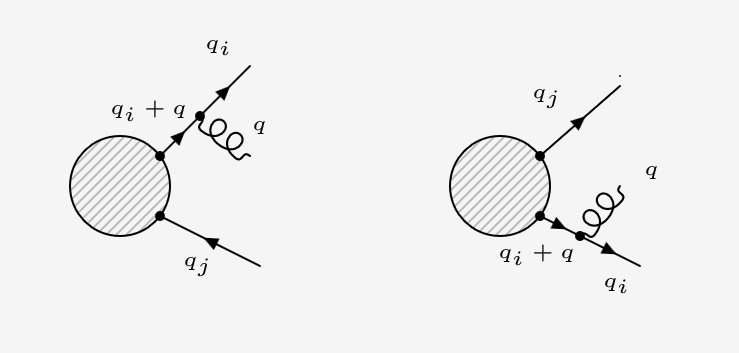
\includegraphics[width=0.85\textwidth]{images/qqg-diagrams.png}
\end{figure}

\subsection{qg-$\bar{q}$}

\begin{figure}[h!]
\centering
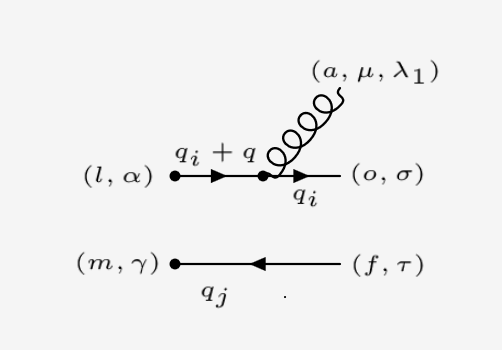
\includegraphics[width=0.85\textwidth]{images/qgqbarM.png}
\end{figure}


\begin{figure}[h!]
\centering
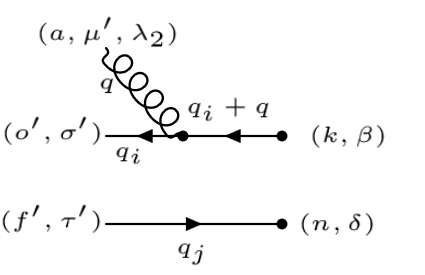
\includegraphics[width=0.85\textwidth]{images/qgqbarMDega.png}
\end{figure}


\begin{figure}[h!]
\centering
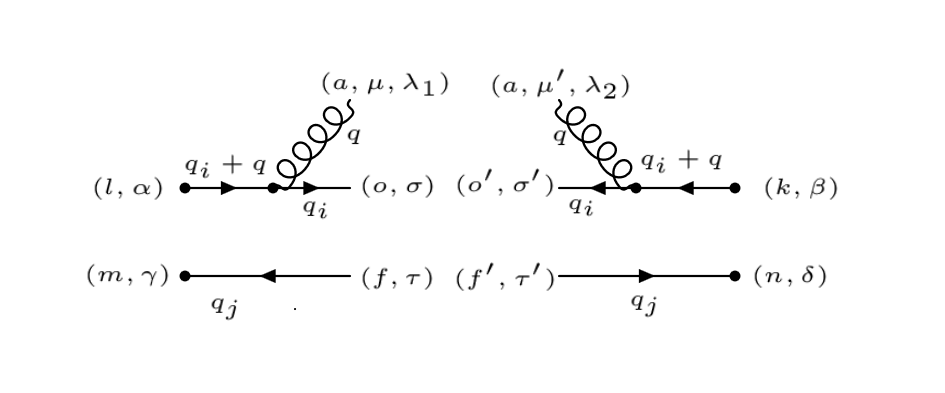
\includegraphics[width=0.85\textwidth]{images/qgqbarMSquer.png}
\end{figure}
\newpage

\subsection{$\bar{q}$g-q}

\begin{figure}[h!]
\centering
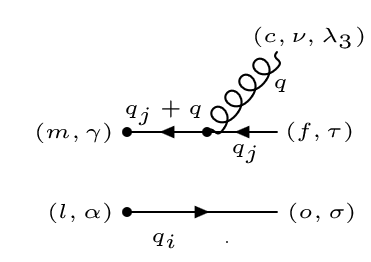
\includegraphics[width=0.85\textwidth]{images/qbargqM.png}
\end{figure}


\begin{figure}[h!]
\centering
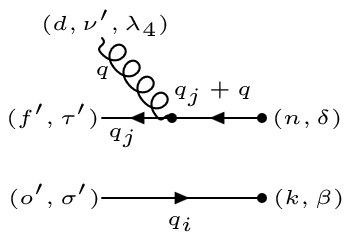
\includegraphics[width=0.85\textwidth]{images/qbargqMDega.png}
\end{figure}


\begin{figure}[h!]
\centering
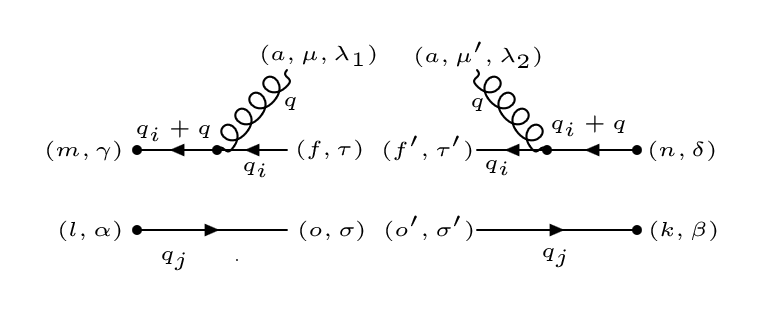
\includegraphics[width=0.85\textwidth]{images/qbargqMSquer.png}
\end{figure}
\newpage

\subsection{$M_1 {M_2}^{\dagger}$}

\begin{figure}[h!]
\centering
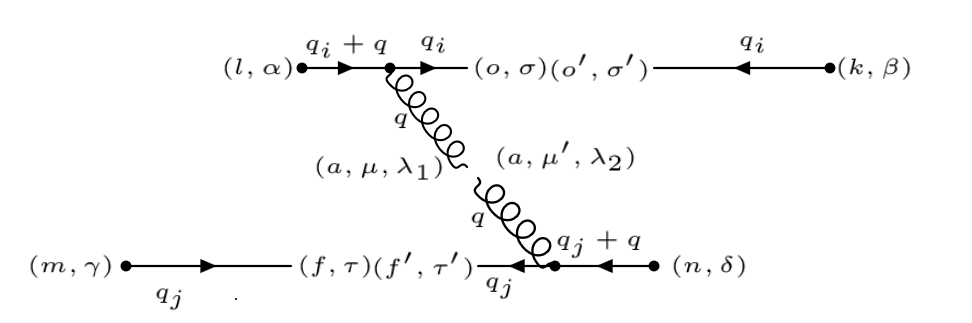
\includegraphics[width=0.85\textwidth]{images/M1M2Degaqqg.png}
\end{figure}

\subsection{$|M^{2}|$}

\begin{figure}[h!]
\centering
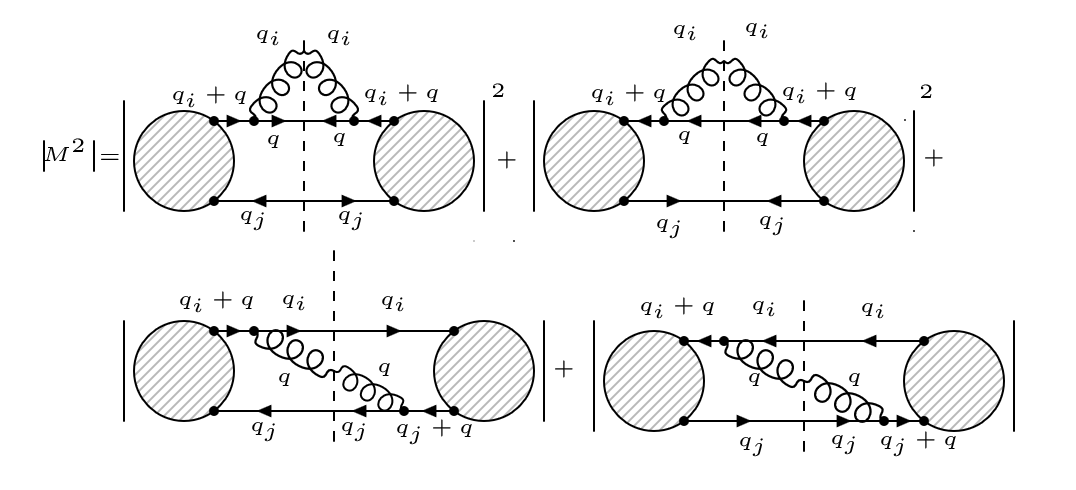
\includegraphics[width=0.85\textwidth]{images/qqgMSquer.png}
\end{figure}

\begin{figure}[h!]
\centering
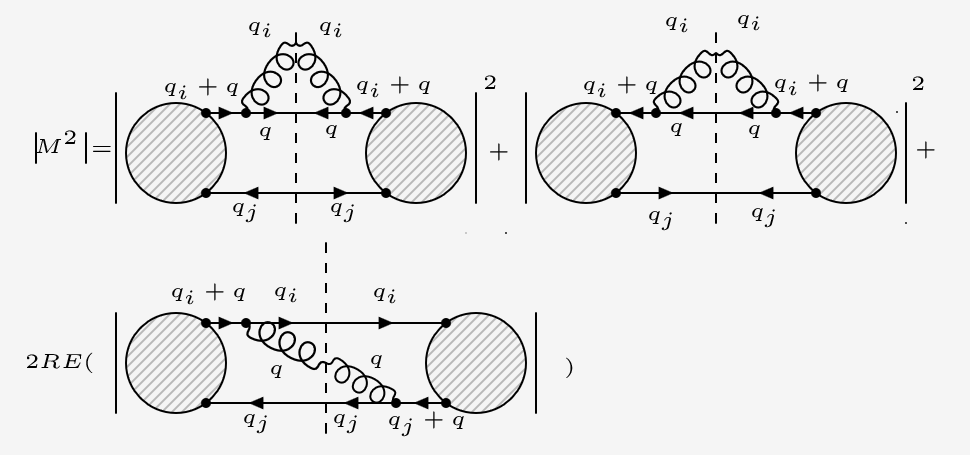
\includegraphics[width=0.85\textwidth]{images/REqqgMSquer.png}
\end{figure}

\newpage
\newpage
 \chapter{Gluon quark gluon emission kernel}
\section{Quark/Gluon gluon emission kernel}

\begin{figure}[ht!]
\centering
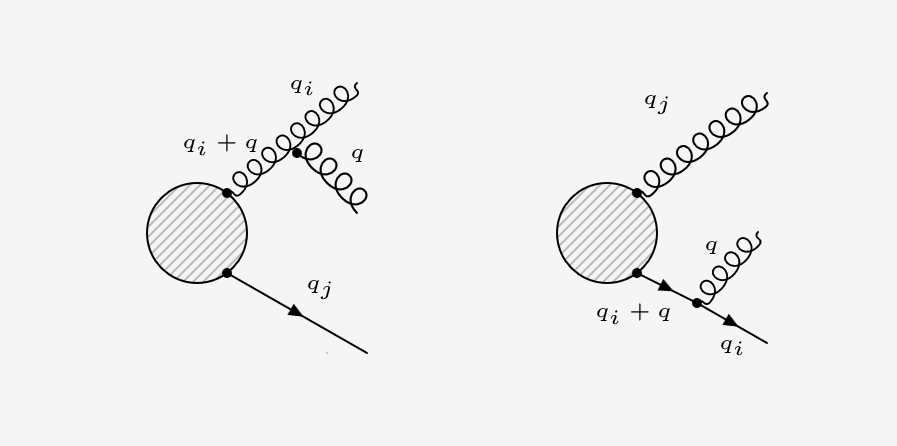
\includegraphics[width=0.85\textwidth]{images/ggq-diagrams.png}
\end{figure}
\subsection{gg-q}
\begin{figure}[ht!]
\centering
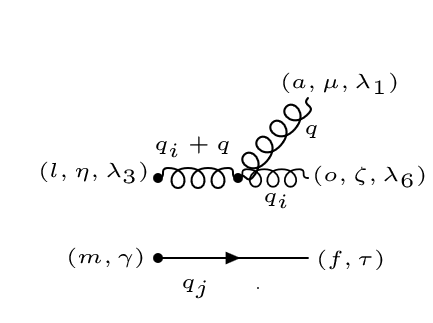
\includegraphics[scale=0.7]{images/ggqM1.png}
\end{figure}
\begin{equation}
\begin{split}
M_1=[\frac{-ig_{{\eta}{\zeta}}}{(q_i +q)^2}(-g_s f^{\:a\:o\:l}(g^{{\mu}{\zeta}}(-q_i +q)^{\eta}+g^{{\zeta}{\eta}}(-q-(q_i +q))^{\mu}+g^{{\eta}{\mu}}(q_i +q+q_i)^{\zeta})\\
{\varepsilon^{\lambda_1}}_{\mu} (q) {\varepsilon^{\lambda_6}}_{\zeta} (q_i)][\bar{u}_{\tau}(q_j)]
\end{split}
\end{equation}

\begin{equation}
\begin{split}
M_1=[\frac{-ig_{{\eta}{\zeta}}}{(q_i +q)^2}(-g_s f^{\:a\:o\:l}(g^{{\mu}{\zeta}}(q-q_i)^{\eta}-g^{{\zeta}{\eta}}(2q_i +q)^{\mu}+g^{{\eta}{\mu}}(2q_i +q)^{\zeta})\\
{\varepsilon^{\lambda_1}}_{\mu} (q) {\varepsilon^{\lambda_6}}_{\zeta} (q_i)][\bar{u}_{\tau}(q_j)]
\end{split}
\end{equation}
\begin{figure}[ht!]
\centering
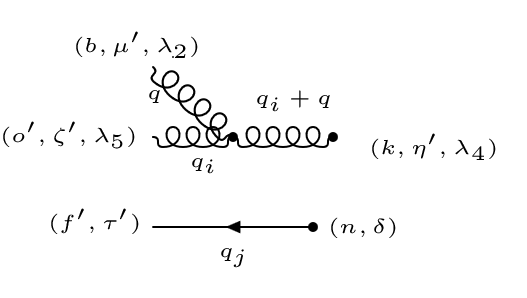
\includegraphics[scale=0.7]{images/ggqM1dagger.png}
\end{figure}
\begin{equation}
\begin{split}
{M_1}^{\dagger}=[\frac{ig_{{{\eta}^{\prime}}{{\zeta}^{\prime}}}}{(q_i +q)^2}(-g_s f^{\:a^{\prime}\:o^{\prime}\:k}(g^{{{\mu}^{\prime}}{{\zeta}^{\prime}}}(q-q_i)^{{\eta}^{\prime}}-g^{{{\zeta}^{\prime}}{{\eta}^{\prime}}}(2q_i +q)^{{\mu}^{\prime}}+g^{{{\eta}^{\prime}}{{\mu}^{\prime}}}(2q_i +q)^{{\zeta}^{\prime}})\\
{{\varepsilon^{\lambda_2}}_{{\mu}^{\prime}}}^* (q) {{\varepsilon^{\lambda_5}}_{{\zeta}^{\prime}}}^* (q_i)][{u}_{{\tau}^{\prime}}(q_j)]
\end{split}
\end{equation}
\begin{figure}[ht!]
\centering
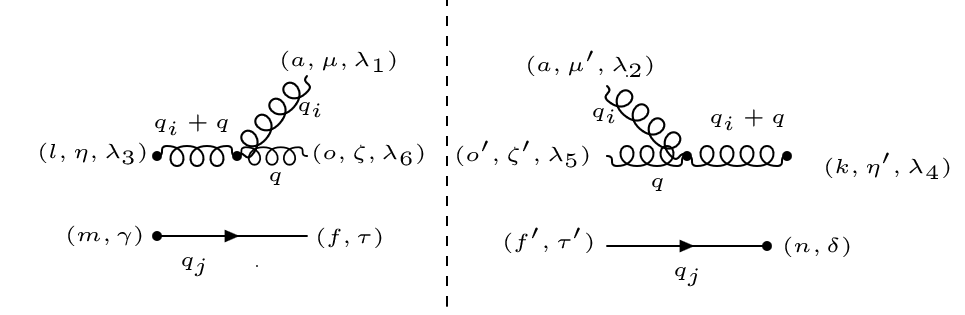
\includegraphics[width=0.95\textwidth]{images/ggqM1squer.png}
\end{figure}
\begin{equation}
\begin{split}
|M_1|^2=[\frac{-ig_{{\eta}{\zeta}}}{(q_i +q)^2}(-g_s f^{\:a\:o\:l}(g^{{\mu}{\zeta}}(-q_i +q)^{\eta}+g^{{\zeta}{\eta}}(-q-(q_i +q))^{\mu}+g^{{\eta}{\mu}}(q_i +q+q_i)^{\zeta})\\
{\varepsilon^{\lambda_1}}_{\mu} (q)\:{{\varepsilon^{\lambda_2}}_{{\mu}^{\prime}}}^* (q) {\varepsilon^{\lambda_6}}_{\zeta} (q_i)\:{{\varepsilon^{\lambda_5}}_{{\zeta}^{\prime}}}^* (q_i)\\
(-g_s f^{\:a^{\prime}\:o^{\prime}\:k}(g^{{{\mu}^{\prime}}{{\zeta}^{\prime}}}(q-q_i)^{{\eta}^{\prime}}-g^{{{\zeta}^{\prime}}{{\eta}^{\prime}}}(2q_i +q)^{{\mu}^{\prime}}+g^{{{\eta}^{\prime}}{{\mu}^{\prime}}}(2q_i +q)^{{\zeta}^{\prime}})\frac{ig_{{{\eta}^{\prime}}{{\zeta}^{\prime}}}}{(q_i +q)^2}][\bar{u}_{\tau}(q_j){u}_{{\tau}^{\prime}}(q_j)]
\end{split}
\end{equation}


\begin{equation}
\begin{split}
|M_1|^2=\frac{{g_s}^2 f^{\:a\:o\:l} f^{\:a^{\prime}\:o^{\prime}\:k}}{(q_i +q)^2 (q_i +q)^2}\\
[g_{{\eta}{\zeta}}(g^{{\mu}{\zeta}}(-q_i +q)^{\eta}+g^{{\zeta}{\eta}}(-q-(q_i +q))^{\mu}+g^{{\eta}{\mu}}(q_i +q+q_i)^{\zeta})\\
g_{{\mu}{{\mu}^{\prime}}} g_{{\zeta}{{\zeta}^{\prime}}}
(g^{{{\mu}^{\prime}}{{\zeta}^{\prime}}}(q-q_i)^{{\eta}^{\prime}}-g^{{{\zeta}^{\prime}}{{\eta}^{\prime}}}(2q_i +q)^{{\mu}^{\prime}}+g^{{{\eta}^{\prime}}{{\mu}^{\prime}}}(2q_i +q)^{{\zeta}^{\prime}})g_{{{\eta}^{\prime}}{{\zeta}^{\prime}}}][\not{q_j}]
\end{split}
\end{equation}
\pagebreak

\subsection{qg-g}
\begin{figure}[ht!]
\centering
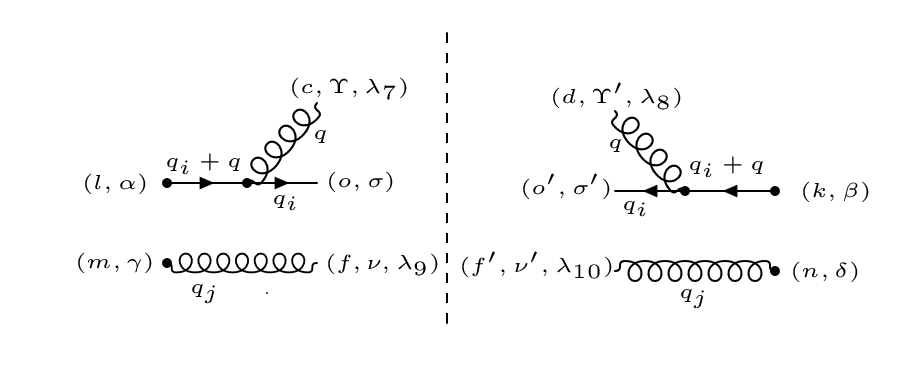
\includegraphics[width=0.95\textwidth]{images/qggM2squer.png}
\end{figure}
\begin{equation}
\begin{split}
|M_2|^2=M_2\:{\color[RGB]{255,0,0} {M_2}^{\dagger}} = [{\bar{u}}_{\sigma}(q_i)\: (-ig_s \gamma^{\mu}\times {[T^c]_o}^l) \: \frac{i(\not{q_i} + \not{q})}{(q_i + q)^2}\:\: {\varepsilon^{\lambda_7}}_{\Upsilon} (q)] [{\varepsilon^{\lambda_9}}_{\nu} (q_j)]\: \\
\quad\quad\quad\quad\quad\quad\quad\quad\:\:{\color[RGB]{255,0,0}[\frac{-i(\not{q_i} + \not{q})}{(q_i + q)^2} \:  (ig_s \gamma^{{\mu}^{\prime}}\times {[T^d]_{o\:^{\prime}}}^k) \: u_{{\sigma}^{\prime}}(q_i) \: {{\varepsilon^{\lambda_8}}_{{\Upsilon}^{\prime}}}^* (q)][{{\varepsilon^{\lambda_{10}}}_{{\nu}^{\prime}}}^* (q_j)]}
\end{split}
\end{equation}

\begin{equation}
\begin{split}
|M_2|^2=[\frac{-i(\not{q_i} + \not{q})}{(q_i + q)^2} \:
 \:  (-ig_s \gamma^{\mu}\times {[T^c]_o}^l) \: {\bar{u}}_{\sigma}(q_i)\:u_{{\sigma}^{\prime}}(q_i) \: {\varepsilon^{\lambda_7}}_{\Upsilon} (q) {{\varepsilon^{\lambda_8}}_{{\Upsilon}^{\prime}}}^* (q) \\
\times (ig_s \gamma^{{\mu}^{\prime}}\times {[T^d]_{o\:^{\prime}}}^k) \: \frac{i(\not{q_i} + \not{q})}{(q_i + q)^2} ]
[{{\varepsilon^{\lambda_{10}}}_{{\nu}^{\prime}}}^* (q_j) {\varepsilon^{\lambda_9}}_{\nu} (q_j)]
\end{split}
\end{equation}

\begin{equation}
\begin{split}
|M_2|^2=\frac{{g_s}^2 {[T^c]_o}^l {[T^d]_{o\:^{\prime}}}^k}{(q_i + q)^2 (q_i + q)^2}
[(\not{q_i} + \not{q}) \:
 \:  \gamma^{\mu} \: \not{q_i} \: (-g_{{\Upsilon}{{\Upsilon}^{\prime}}}) \\
\gamma^{{\mu}^{\prime}} \: (\not{q_i} + \not{q})]
[-g_{{\nu}^{\prime}{\nu}}]
\end{split}
\end{equation}

\subsection{$M_1 {M_2}^{\dagger}$}
\begin{figure}[ht!]
\centering
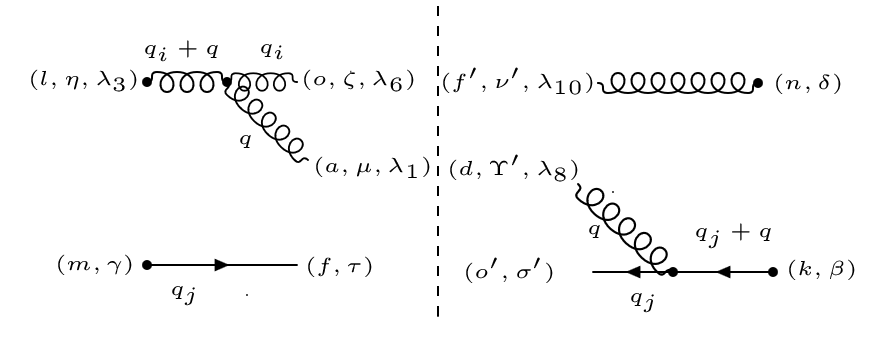
\includegraphics[width=0.95\textwidth]{images/ggqM1M2dagger.png}
\end{figure}
\begin{equation}
\begin{split}
M_1\:{\color[RGB]{255,0,0} {M_2}^{\dagger}}=[\frac{-ig_{{\eta}{\zeta}}}{(q_i +q)^2}(-g_s f^{\:a\:o\:l}(g^{{\mu}{\zeta}}(q-q_i)^{\eta}-g^{{\zeta}{\eta}}(2q_i +q)^{\mu}+g^{{\eta}{\mu}}(2q_i +q)^{\zeta})\\
{\varepsilon^{\lambda_1}}_{\mu} (q_i) {\varepsilon^{\lambda_6}}_{\zeta} (q)][\bar{u}_{\tau}(q_j)]
{\color[RGB]{255,0,0}[\frac{-i(\not{q_j} + \not{q})}{(q_j + q)^2} \:  (ig_s \gamma^{{\mu}^{\prime}}\times {[T^d]_{o\:^{\prime}}}^k) \: u_{{\sigma}^{\prime}}(q_j) \: {{\varepsilon^{\lambda_8}}_{{\Upsilon}^{\prime}}}^* (q)][{{\varepsilon^{\lambda_{10}}}_{{\nu}^{\prime}}}^* (q_i)]}
\end{split}
\end{equation}









%\begin{equation}
%\begin{split}
%M_1\:{M_2}^{\dagger}=\frac{{g_s}^2 f^{\:a\:o\:l} {[T^d]_{o\:^{\prime}}}^k}{(q_i + q)^2 (q_j + q)^2}\\
%
%[g_{{\eta}{\zeta}}(g^{{\mu}{\zeta}}(q-q_i)^{\eta}-g^{{\zeta}{\eta}}(2q_i +q)^{\mu}+g^{{\eta}{\mu}}(2q_i +q)^{\zeta})\\
%g_{{\mu}{\zeta}}][(\not{q_j} + \not{q})\:\gamma^{{\mu}^{\prime}}\:\not{q_j} {{\varepsilon^{\lambda_8}}_{{\Upsilon}^{\prime}}}^* (q)][{{\varepsilon^{\lambda_{10}}}_{{\nu}^{\prime}}}^* (q_i)]
%\end{split}
%\end{equation}


\pagebreak

\subsection{$|M^{2}|$}
\begin{figure}[ht!]
\centering
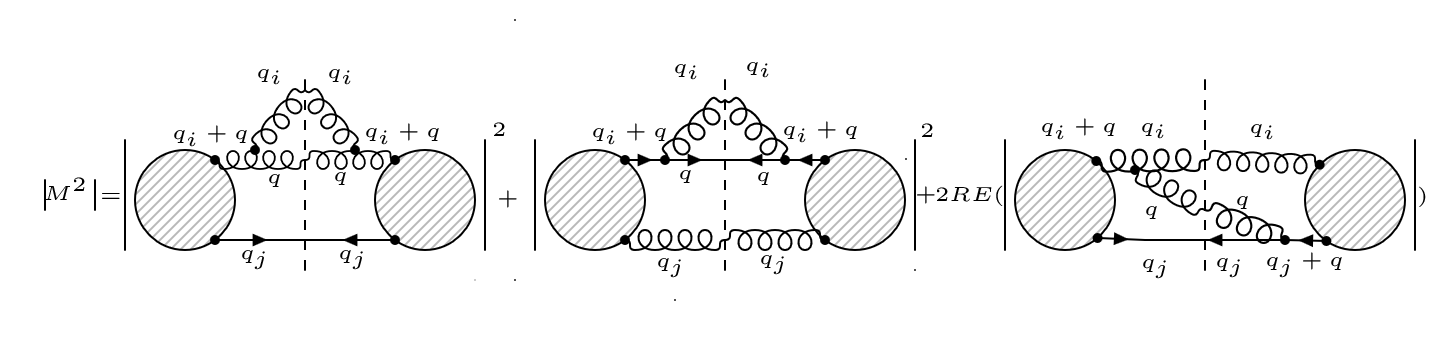
\includegraphics[width=1.0\textwidth]{images/ggq-MSquerRE.png}

\end{figure}
   
      
\bibliographystyle{plain}
\bibliography{bibliography2}


%\listoftables
%\listoffigures
%\printindex

\appendix

First of all I would like to thank all those who supported me during the preparation of this work and who contributed a lot to the success of this work, in particular:\\
\\
PD Dr. Stefan Gieseke for his excellent care and patience.\\
\\
Prof. Dr. Dieter Zeppenfeld for the takeover of the second assessor.\\
\\
Dr. Simon Plätzer who gave me a helpful feedback and took the time to discuss this work.\\
My great thanks also go to Emma Simpson Dore, who proofread my work in numerous hours. She pointed out to me the weaknesses of my letter and showed me the right paths to reach my goal at work.\\
\\ 
Finally, I would like to thank my girlfriend Canan Kaman, who supported me in all things in this not always easy time.\\


 
         


 


\end{document}
